\documentclass[12pt]{jarticle}
%\documentclass[12pt, draft]{jarticle}  % 図の出力を省略.最後に直す.
%\documentstyle[12pt,fleqn,epsf,iepaper,cite]{jarticle}
%\documentstyle[12pt,iepaper,eclepsf,oddchar]{jarticle}
\usepackage[dvipdfm]{graphicx}
\usepackage{iepaper}
\usepackage{epsf}
\usepackage{ccaption}


%%%%%%%%%%%%%%%%%%%%%%%%%%%%%%
%%% added by tada
\usepackage{url}
\usepackage{multirow}
\usepackage{afterpage}
%\usepackage[hang,small,bf]{caption}
\usepackage[subrefformat=parens]{subcaption}
\captionsetup{compatibility=false}
% end


%%%%%%%%%%%%%%%%%%%%%%%%%%%%%%
% タイトル改行した方が良い?
\title{皮肉データセットを用いた深層学習による\\皮肉推定手法}
\author{多田 瑞葵}
\gakuseki{1181201087}[B]  %\UTF{FFFD}\UTF{FFFD}\UTF{FFFD}_\UTF{FFFD}\UTF{FFFD}B\UTF{FFFD}C\UTF{FFFD}C\UTF{FFFD}_\UTF{FFFD}\UTF{FFFD}M  gakubu = B, syuushi = M ?
\group{第 1 研究グループ}            % \UTF{FFFD}\UTF{FFFD}\UTF{FFFD}_\CID{1466}\UTF{A347}%
\shidou{森 直樹 教授}                          % \UTF{FFFD}\UTF{FFFD}\UTF{FFFD}_\CID{1466}\UTF{A347}%
%\syusa{\UTF{FFFD}\UTF{FFFD}\UTF{FFFD}\UTF{FFFD}}                            % \UTF{FFFD}C\UTF{FFFD}_\CID{1466}\UTF{A347}%
%\hukusa{\UTF{FFFD}\UTF{FFFD}\UTF{FFFD}\UTF{FFFD}}{\UTF{FFFD}\UTF{FFFD}\UTF{FFFD}\UTF{FFFD}}

%\UTF{FFFD}}\UTF{FFFD}\UTF{050D}\UTF{FFFD}\UTF{FFFD}\UTF{FFFD}\UTF{FFFD}u(section\UTF{FFFD}\UTF{050D}\UTF{FFFD}).(\UTF{FFFD}}\UTF{FFFD}\UTF{050D}\UTF{FFFD})\UTF{FFFD}v\UTF{FFFD}\UTF{0182}\UTF{FFFD}\UTF{FFFD}\UTF{90BD}\UTF{FFFD}\UTF{FFFD}%
\makeatletter
 \renewcommand{\thefigure}{%
   \thesection.\arabic{figure}}
  \@addtoreset{figure}{section}
\makeatother

\makeatletter
 \renewcommand{\thetable}{%
   \thesection.\arabic{table}}
  \@addtoreset{table}{section}
\makeatother

\makeatletter
 \renewcommand{\theequation}{%
   \thesection.\arabic{equation}}
  \@addtoreset{equation}{section}
\makeatother


\begin{document}
\maketitle
\pagenumbering{roman}  % page numbering i, ii
%%% \UTF{FFFD}\UTF{068E}\UTF{FFFD}%
\tableofcontents  % mokuji
\newpage
%

%% \UTF{FFFD}}\UTF{FFFD}\UTF{A5D7}%
\listoffigures  % zu ichiran
\newpage

%% \UTF{FFFD}\\UTF{FFFD}\UTF{A5D7}%
 \listoftables  % hyou ichiran
 \newpage

\pagenumbering{arabic}  % page numbering 1, 2

% \UTF{FFFD}\UTF{FFFD}\UTF{FFFD}\UTF{FFFD}\UTF{FFFD}J\UTF{FFFD}n
%\include{./doc/99_memo}  % memo, ato de sakujo suru
%\clearpage

% 1. introduction
\newpage
\changeindent{0cm}
\section{はじめに}
\changeindent{2cm}


計算機による文章の理解において,様々な修辞表現の理解が重要な課題となっている.
修辞表現の一つである皮肉表現は,文章の文字通りの意味と書き手の意図とが異なる言語表現である.
人間の場合,ある文章が皮肉であるか否かを推定することは凡そ容易である.
一方で,文章を文字情報に基づいて処理する場合,皮肉推定は困難である.
そのため,計算機による皮肉推定は,文章の理解や創作,感情分析等の分野でも解決すべき課題となっている.
\par
皮肉の表現の幅は広く,全ての皮肉表現を一括りに扱って推定することは良策ではない.
そこで本研究では,皮肉推定の前段階として,文章の話題ごとの皮肉推定に取り組んだ.
ソーシャルメディアサイト Reddit には,subreddit と呼ばれる投稿トピックがある.
この subreddit のそれぞれについて皮肉推定をし,その結果を分析することにより,文章の話題ごとの皮肉推定の有効性を検証した.
また,モデルには深層言語モデル BERT を使用することで,文脈を考慮した皮肉推定に取り組んだ.
\par
本稿では,まず第 2 章で皮肉推定に関する関連研究を紹介する.続いて第 3 章で本研究で使用した要素技術とデータセットについて記述する.第 4 章では本研究で取り組んだ実験について記述する.

\clearpage

%% 2. previous research
\newpage
\changeindent{0cm}
\section{関連研究}
\changeindent{2cm}



本章では皮肉表現の心理的・言語的側面の研究と,計算機による皮肉推定に関連する研究を紹介する.
\par

%%%%%%%%%%%%%%%%%%%%%%%%%%%%%%
\subsection{皮肉表現の心理的・言語的研究}

人間にとって,ある発話や文章が皮肉であることを理解するのは容易であるが,その現象を説明することは難しい \cite{GIBBS1991523}.
例えば,相手がその文章によって伝えたいことを理解する際に,その文章に皮肉表現が含まれていることを認識する必要はないことから,人間は無意識に皮肉を理解できると言える.
さらに話し手や書き手が皮肉を意図していなくても,受け取る側によって皮肉であると解釈されることがある.
これらは皮肉表現の心理的側面に焦点を当てた説明である.
言語的側面からは,皮肉表現は語用論的原則の違反によって説明されることがある \cite{HAVERKATE199077}.
これは皮肉表現が文章の文字通りの意味と書き手の意図とが異なる言語表現であるという説明を含んでいる.
以上のように皮肉表現は多角的に研究されているが,全ての皮肉表現を説明しきる理論は未だ存在しない \cite{Ozerova}.


%%%%%%%%%%%%%%%%%%%%%%%%%%%%%%
\subsection{皮肉推定のためのデータセット}

皮肉推定の研究に利用されているデータセットにはソーシャルネットワーキングサービスに投稿された文章を収集したものが多い.
特に Twitter \footnote{\url{https://about.twitter.com/en}} に投稿された文章(ツイート)を収集し,皮肉推定に使用している研究は多く見られる.
Riloff らは皮肉を明示するハッシュタグ “\#sarcasm ”,“\#sarcastic” を手がかりに皮肉データを収集した \cite{DBLP:conf/emnlp/RiloffQSSGH13}.
一方で Ghosh \& Veale はハッシュタグだけを手がかりとするとタグ付けされていないデータを収集できないことを指摘している \cite{ghosh-veale-2017-magnets}.彼らは Twitterbot を用いて,皮肉と思われるツイートに対して投稿者に直接確認を取ることで皮肉データを収集した.
\par
News Headlines Dataset For Sarcasm Detection \cite{misra2019sarcasm} は,ウェブニュースサイト TheOnion \footnote{\url{https://www.theonion.com}} と HuffPost \footnote{\url{https://www.huffpost.com}} からヘッドラインを収集したデータセットである.
TheOnion は時事問題に対して皮肉的なヘッドラインを付けることで有名である.
そのため TheOnion から収集したヘッドラインデータに皮肉ラベルを,HuffPost から収集したデータに非皮肉ラベルを付与している.
ヘッドラインのみのデータであるため各データに文脈が存在せず,1 つの文章で理解可能な皮肉表現となっている.



%%%%%%%%%%%%%%%%%%%%%%%%%%%%%%
\subsection{SARC データセットを用いた皮肉推定}
本研究では SARC データセット \cite{khodak2018} を用いて皮肉推定をした.
このデータセットの特徴として Twitter データセットやヘッドラインデータセットと比べて大規模であることが挙げられる.
またメタデータも充実しており,近年の皮肉表現に関する研究に大きく貢献しているデータセットである.
本節ではこのデータセットを用いた関連研究を紹介し,SARC データセットについては後の章で詳述する.
\par


%\par
%%%%%%%%%%%%%%%%%%%%%%%%%%%%%%
% 2018 05 CASCADE: Contextual Sarcasm Detection in Online Discussion Forums
2018 年に,ソーシャルメディアサイトへの投稿文章に対する皮肉推定のモデルとして CASCADE \cite{hazarika-etal-2018-cascade} が提案され,state-of-the-art を達成した.
このモデルは文章の情報に加えて,投稿者と投稿トピックを元にした情報を特徴量として利用する.
具体的には,Convolutional Neural Network (CNN) を用いて取得した文章の分散表現 $\overrightarrow{c}_{i,j}$,投稿者の過去の投稿文章から取得した分散表現 $\overrightarrow{u}_{i}$,投稿トピックにおける投稿文章から取得した分散表現 $\overrightarrow{t}_{j}$ を連結して分類に用いている.
結果として,文章の情報と投稿者や投稿トピックを元にした情報を併用することで,皮肉推定の精度が向上することを示した.


\par
%%%%%%%%%%%%%%%%%%%%%%%%%%%%%%
% 2019 Deep and Dense Sarcasm Detection
文章の情報のみを使用した研究もされている.
2019 年に Pelser \& Murrell \cite{pelser2019deep} は,投稿者などの情報はプライバシー設定やデータ欠損により常に利用可能とは限らないことを指摘し,56 層の深層ネットワークによる文章のみを利用した推定手法を提案した.
結果として,上述した CASCADE の性能を上回ることはできなかったものの,文章以外の情報を利用した他の既存手法に匹敵する性能を示した.


\par
%%%%%%%%%%%%%%%%%%%%%%%%%%%%%%
本研究では文章情報からの皮肉推定に重きを置くため投稿者の情報は使用しない.
また subreddit の情報を使用することで話題ごとの皮肉推定の有効性を確認する.








\clearpage

% 3. method
\newpage
\changeindent{0cm}
\section{要素技術}
\changeindent{2cm}


%%%%%%%%%%%%%%%%%%%%%%%%%%%%%%
% 3.1. BERT
% https://arxiv.org/abs/1810.04805
% 3.2 SARC データセット
%%%%%%%%%%%%%%%%%%%%%%%%%%%%%%
本章では,本研究で使用した要素技術とデータセットについて記述する.
\subsection{BERT}

Bidirectional Encoder Representations from Transformers (BERT) \cite{devlin-etal-2019-bert} は,2018 年 10 月に Jacob Devlin らが発表した Transformer \cite{NIPS2017_3f5ee243} による双方向のエンコーダーを用いた言語モデルである.
公開当時に様々な自然言語処理タスクで state-of-the-art の性能を示した.
文章を文頭と文末の双方向から学習することによって文脈の理解を可能としている.
\par 
BERT は大規模コーパスを用いて事前学習することでモデルの性能を向上させている.
事前学習には,[MASK] トークンに当てはまる単語を予測する Masked Language Modeling と,入力された 2 文が意味的に連続するかを予測する Next Sentence Prediction の 2 つのタスクが用いられる.
\par
BERT は様々な事前学習済みモデルが発表されており,ファインチューニングすることで各タスクに応用可能である.
図 \ref{fig:31_bert_model} はその概略図を表している.
本研究では,英語の事前学習済みモデルである bert-base-uncased \footnote{\url{https://huggingface.co/bert-base-uncased}} を使用した.
このモデルは本のデータセットである BookCorpus \cite{bookcorpus} と Wikipedia \footnote{\url{https://en.wikipedia.org/wiki/Main_Page}} の英語記事を用いて事前学習している.
BookCorpus は約 8 億語,Wikipedia は約 2 億 5 千万語を含んでいる.
またこのモデルは英語の大文字と小文字の区別をしない.
モデルの層数は 12 層,隠れ層の次元数は 768 次元,最大入力長は 512 トークンである.


%%% figure BERT のファインチューニング
\begin{figure}[b]
 	\begin{center}
		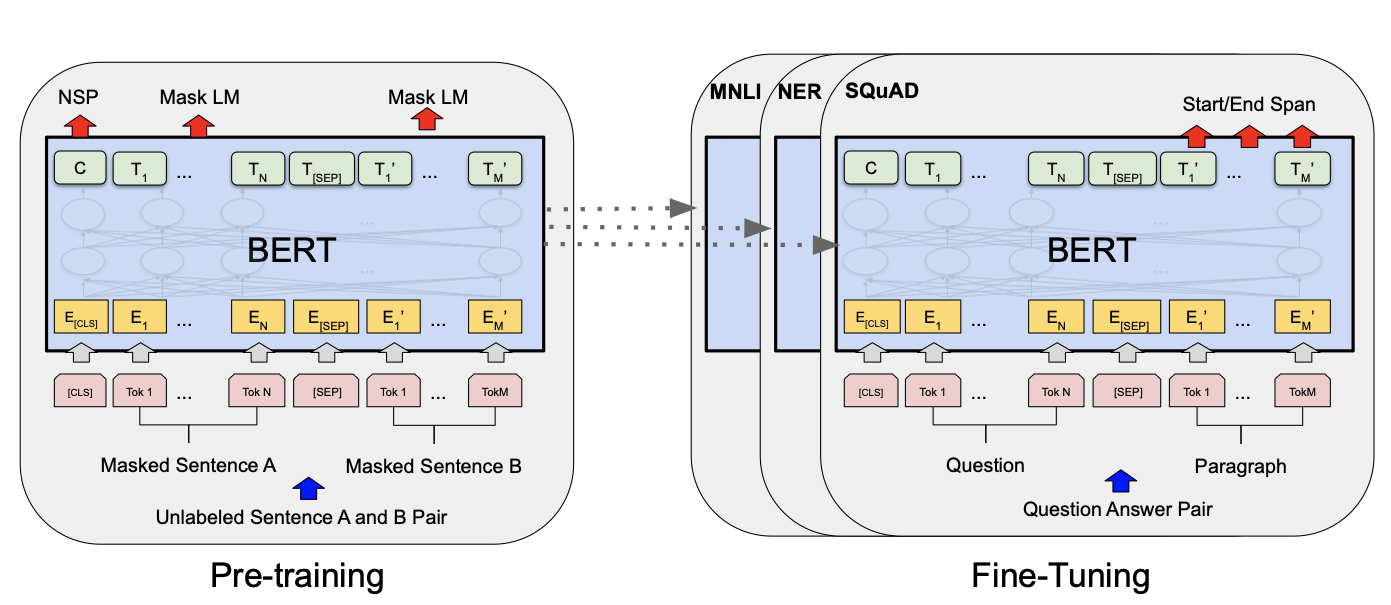
\includegraphics[width=\linewidth]{./figure/31_BERT_figure1.png}
		\caption{BERT のファインチューニングの概要図(文献 \cite{devlin-etal-2019-bert} Figure 1 より引用)}
		\label{fig:31_bert_model}
	\end{center}
\end{figure}
% end figure

BERT に文を入力する際は,まず tokenizer を用いて文をトークンに分割し,ID に変換する.
本研究では BERT モデルと同じ bert-base-uncased の tokenizer を使用した.
この tokenizer は WordPiece \cite{wu2016googles} モデルを用いて,文を単語よりも細かいサブワードに分割する.
これによって未知語を分解し,削減することができる.
BERT には特殊トークンが用意されており,入力の際は変換した ID 列の先頭に [CLS] トークンを,各文の末尾に該当する位置に [SEP] トークンを挿入する.
入力に対して BERT は各トークンに対応する分散表現を出力する.
このとき [CLS] トークンに対応する分散表現は入力された文全体の特徴を捉えており,分類問題に使用することができる.

%\newpage
%\changeindent{0cm}
%\section{要素技術}
%\changeindent{2cm}


%%%%%%%%%%%%%%%%%%%%%%%%%%%%%%
% 3.1. BERT
% 3.2 Optuna
% 3.3 SARC データセット
%%%%%%%%%%%%%%%%%%%%%%%%%%%%%%
\subsection{Optuna}
% https://www.preferred.jp/ja/projects/optuna/
% https://github.com/optuna/optuna
% https://arxiv.org/pdf/1907.10902.pdf
% https://tech.preferred.jp/ja/blog/optuna-release/


Optuna \cite{akiba2019optuna} は,オープンソースのハイパーパラメータ自動最適化フレームワークである.
Tree-structured Parzen Estimator というベイズ最適化アルゴリズムを用いて,過去の試行に基づいて有望そうな領域を推定し再度試行する.
これを繰り返すことで最適なハイパーパラメータの値を自動的に発見する.
使用する際は目的関数を定め,その値がより大きくまたは小さくなるように推定を進める.
Optuna の主な特徴として,Define-and-Run スタイルの API,学習曲線を用いた試行の枝刈り,並列分散最適化が挙げられる.


%\newpage
%\changeindent{0cm}
%\section{要素技術}
%\changeindent{2cm}


%%%%%%%%%%%%%%%%%%%%%%%%%%%%%%
% 3.1. BERT
% 3.2 SARC データセット
%%%%%%%%%%%%%%%%%%%%%%%%%%%%%%
\subsection{SARC データセット}
本研究では,皮肉の研究や皮肉検出システムの学習・評価のための大規模コーパスである,自己注釈付き Reddit コーパス(Self-Annotated Reddit Corpus; SARC)\cite{khodak2018} を使用した.
このデータセットはソーシャルメディアサイト Reddit に投稿されたコメントから構築されている.
図 \ref{fig:reddit_sample} に Reddit に投稿されたコメントの例を示す.
図の上のコメントは投稿元であり,下のコメントはその投稿元に反応したものである.
\par
図 \ref{fig:30_dataset_sample} に SARC データセットに含まれるコメントの例を示す.
各コメントには文章だけではなく,投稿者の識別子,subreddit と呼ばれる投稿トピック,ユーザ評価(good/bad),投稿日時,親投稿の情報も付与されている.
親投稿とは,最初の投稿から各コメントに至るまでの一連の投稿であり,全てのコメントは 1 つ以上の親投稿を保持している.
SARC データセットはこのようなやりとりのうち,末端のコメントのみに皮肉か非皮肉かのラベルが付与されている.
\par

%%% figure Reddit の投稿例
\begin{figure}[b]
 	\begin{center}
		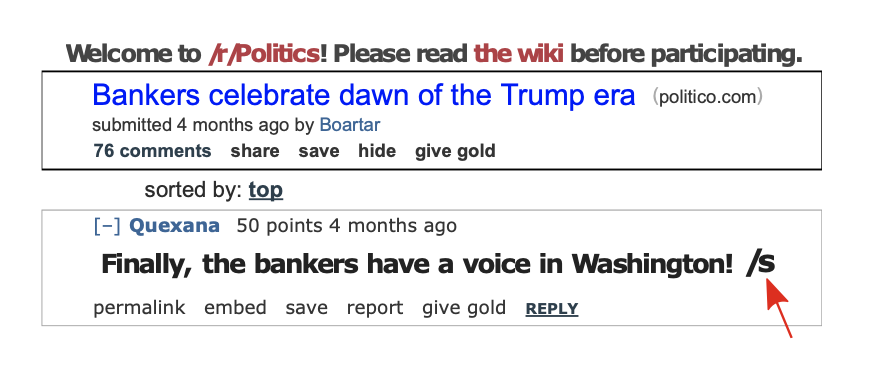
\includegraphics[width=0.8\linewidth]{./figure/30_reddit.png}
		\caption{Reddit に投稿されたコメントの例(文献 \cite{khodak2018} Figure 1 より引用)}
		\label{fig:reddit_sample}
	\end{center}
\end{figure}
% end figure

%%% figure データの例
\begin{figure}[tb]
 	\begin{center}
		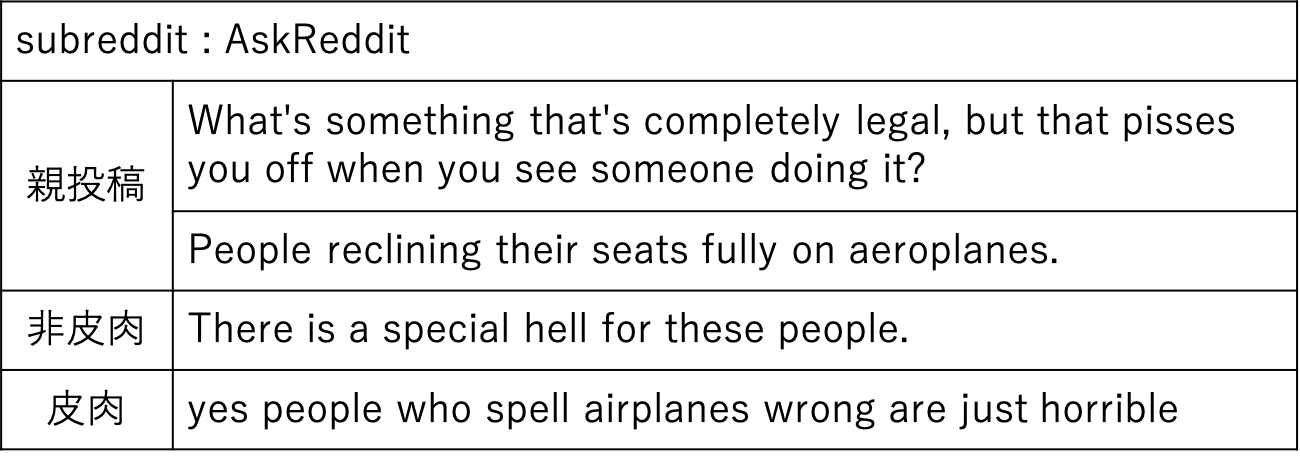
\includegraphics[width=0.8\linewidth]{./figure/30_dataset_sample.png}
		\caption{SARC データセットのデータの例}
		\label{fig:30_dataset_sample}
	\end{center}
\end{figure}
% end figure

Reddit へ投稿する際,ユーザは自分のコメントが皮肉を意図していることを明示する記号 “/s” を使用する.
このことを利用し,投稿コメントに “/s” を含むことを必要条件としてデータに皮肉ラベルが付けられている.
すなわち SARC データセットは,投稿者が皮肉を意図しているかどうかを判断基準としてラベル付けしていると言える.
ただしこの記号は,データセットに含まれる文章からは除去されている.
\par
またこのデータセットには,全ての subreddit からデータを抽出した main データセットと,politics の subreddit からデータを抽出した pol データセットがある.
それぞれに対して均衡データセット(balanced)と不均衡データセット(unbalanced)が用意されており,全部で 4 つのデータセットが用意されている.
均衡データセットには,同じ親投稿に対して 2 つのコメントが存在する.
そして 2 つのコメントの内訳は,皮肉データと非皮肉データが 1 つずつである.
本研究では SARC 2.0 main balanced \footnote{https://nlp.cs.princeton.edu/SARC/2.0/main/} データセットを使用した.
このデータセットに含まれる訓練データは 257,082 件,テストデータは 64,666 件である.
\par
次に,使用したデータセットの subreddit の情報について述べる.訓練データに含まれる subreddit は 4,902 種類,テストデータに含まれる subreddit は 2,666 種類,訓練データとテストデータに共通する subreddit は 2,194 種類であった.
表 \ref{tb:1_subreddit_data} に subreddit ごとのデータ数を示す.
データ数が最も多い subredit は politics で,訓練データ 13,668 件,テストデータ 3,406 件であった.
またデータ数が最も少ない subreddit は複数あり,データ数は 2 件であった.


%%% table subreddit の分布
\begin{table}[tb]
  \caption{subreddit ごとのデータ数の分布}
  \label{tb:1_subreddit_data}
  \centering
  \begin{tabular}{c c c c c} \hline

\multicolumn{3}{c}{データ (件)} & \multicolumn{2}{c}{subreddit (種類)} \\ \cline{4-5}
\multicolumn{3}{c}{(以上) - (未満)} & 訓練 & テスト \\ \hline

& - & 100 & 4,575 & 2,567 \\
100 & - & 500 & 248 & 77 \\
500 & - & 1,000 & 40 & 13 \\
1,000 & - & 2,000 & 17 & 6 \\
2,000 & - & 3,000 & 6 & 1 \\ 
3,000 & - & 4,000 & 7 & 2 \\
4,000 & - & 5,000 & 4 & 0 \\
5,000 & - & 6,000 & 1 & 0 \\
6,000 & - & 7,000 & 0 & 0 \\
7,000 & - & 8,000 & 1 & 0 \\
8,000 & - & 9,000 & 0 & 0 \\
9,000 & - & 10,000 & 1 &  0 \\
10,000 & - & & 2 & 0 \\ \hline
\multicolumn{3}{c}{合計} & 4,902 & 2,666 \\ \hline 

  \end{tabular}
\end{table}
% end






\clearpage

% 4. experimental results
\newpage

\changeindent{0cm}
\section{実験}
\changeindent{2cm}

%%%%%%%%%%%%%%%%%%%%%%%%%%%%%%
%\afterpage{\clearpage}
\subsection{実験 1}

文章の話題ごとに皮肉か非皮肉かを推定する実験に取り組んだ.
モデルには BERT を使用し,データセットには SARC 2.0 main balanced データセットを使用した.
\par
まず subreddit ごとにデータを抽出し,新たにデータセットを作成した.
その際にテストデータが 1,500 件以上取得できたものを選択し,politics,AskReddit,worldnews,pcmasterrace の 4 つのデータセットを実験に使用した.
また比較のため,全ての subreddit からランダムにデータをサンプリングした random データセットを作成し実験に使用した.
このとき同じ親投稿を持つ皮肉データと非皮肉データのペアは崩さないように抽出した.
random データセットに含まれる subreddit を確認したところ,訓練データは 1,257 種類,テストデータは 569 種類の subreddit から構成されていた.
表 \ref{tb:4_subreddit_data} に各データセットのデータ数を示す.
なお各データセットには皮肉データと非皮肉データは同数含まれている.

%%% table
\begin{table}[b]
  \caption{各データセットのデータ数}
  \label{tb:4_subreddit_data}
  \centering
  \begin{tabular}{c c c} \hline

データセット & 訓練 (件) & テスト (件) \\ \hline
politics & 13,668 & 3,406 \\
AskReddit & 11,660 & 3,006 \\
worldnews & 9,444 & 2,246 \\
pcmasterrace & 7,400 & 1,772 \\
random & 14,000 & 3,500 \\ \hline

  \end{tabular}
\end{table}
% end

\par
図 \ref{fig:40_model} にモデルの概要を示す.
まず入力の先頭に [CLS] トークンを,各コメントの末尾に [SEP] トークンを付けて BERT に入力し,分散表現を取得した.
分散表現のうち,文頭の [CLS] トークンに該当する分散表現を入力文章全体の分散表現とみなし,それを線形層に入力して皮肉か非皮肉かを二値分類した.
訓練データでモデルを学習し,テストデータでその性能を評価した.
評価指標には Accuracy(正解率),Precision(適合率),Recall(再現率),F1 値を使用した.

% figure model
 \begin{figure}[tb]
 	\begin{center}
	 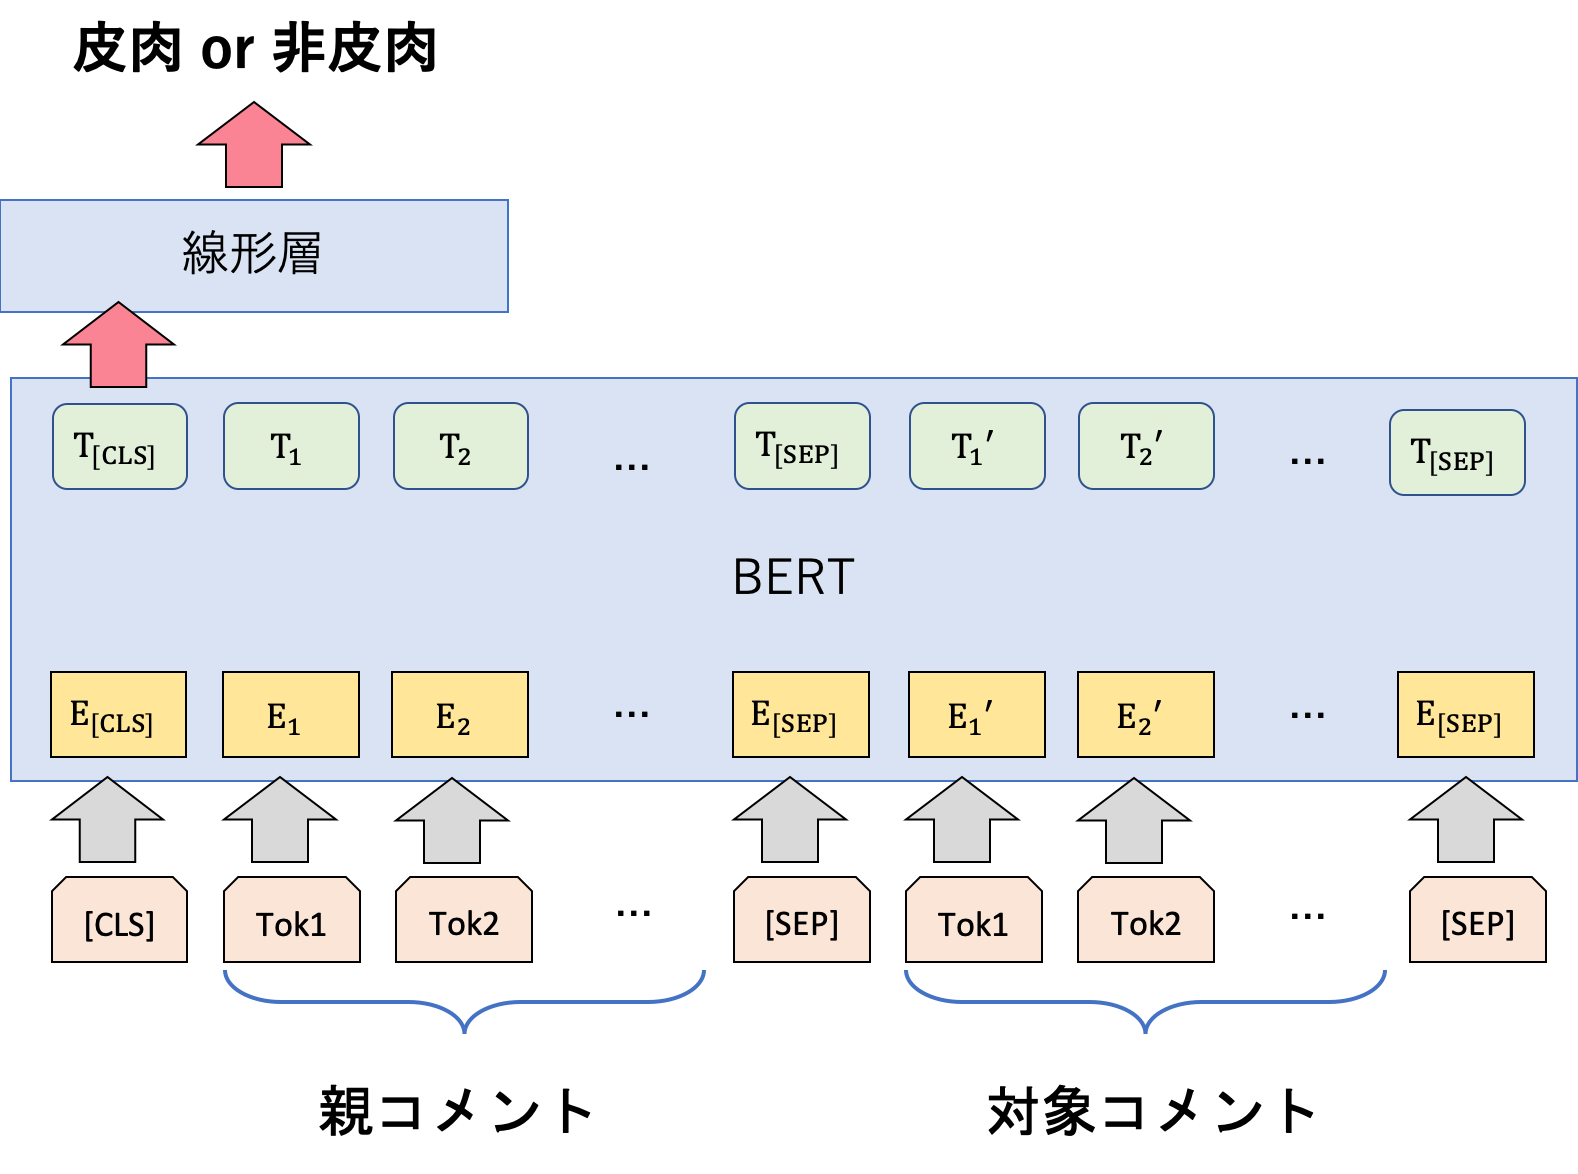
\includegraphics[width=0.8\linewidth]{./figure/40_model.png}
	 \end{center}
 \caption{実験モデルの概要}
 \label{fig:40_model}
 \end{figure}
% end figure


表 \ref{tb:4_bert_param} に実験のパラメータを示す.
BERT と線形層の学習率は予備実験によって値の範囲を定め,Optuna \cite{akiba2019optuna} によって探索した.
学習時は BERT の全層をファインチューニングし,線形層も重みを更新した.
\par

%%% table
\begin{table}[tb]
  \caption{実験パラメータ}
  \label{tb:4_bert_param}
  \centering
  \begin{tabular}{c c} \hline

\multicolumn{2}{c}{BERT} \\ \hline
モデル & bert-base-uncased \\ 
入力層次元数 & 512 \\
出力層次元数 & 768 \\
学習率 & $1 \times 10^{-6}$ 〜 $1 \times 10^{-4}$ \\ \hline
\multicolumn{2}{c}{線形層} \\ \hline
入力層次元数 & 768 \\
出力層次元数 & 2 \\
学習率 & $1 \times 10^{-6}$ 〜 $1 \times 10^{-4}$ \\ \hline
\multicolumn{2}{c}{学習} \\ \hline
エポック数 & 20 \\
バッチサイズ & 16 \\
損失関数 & Cross Entropy Loss \\
最適化関数 & Adam \\
 & $\left( 
 \begin{tabular}{c}
 \footnotesize{learning rate = 0.001} \\ \footnotesize{$\beta_1 = 0.9$, $\beta_2 = 0.999$}
 \end{tabular}
  \right)$ 
%最適化関数 & 
%	\begin{tabular}{c}
%	Adam \\ learning rate $= 0.001$ \\ $\beta_1 = 0.9$, $\beta_2 = 0.999$
%	\end{tabular}

\\ \hline
  \end{tabular}
\end{table}
% end



%%%%%%%%%%%%%%%%%%%%%%%%%%%%%%
\afterpage{\clearpage}
\subsection{実験 1 結果}
表 \ref{tb:4_bert_result} に実験結果を示す.
太字の項目はベースラインである random データセットでの評価値を上回ったことを表している.

%%% table
\begin{table}[tb]
  \caption{実験結果}
  \label{tb:4_bert_result}
  \centering
  \begin{tabular}{c c c c c} \hline

dataset & Accuracy & Precision & Recall & F1 score  \\ \hline
politics & \textbf{0.730} & \textbf{0.722} & \textbf{0.748} & \textbf{0.735} \\
AskReddit & 0.619 & 0.630 & 0.580 & 0.604 \\
worldnews & \textbf{0.690} & 0.655 & \textbf{0.803} & \textbf{0.721} \\
pcmasterrace & 0.648 & 0.635 & \textbf{0.698}  & \textbf{0.665} \\ \hline
random & 0.653 & 0.664 & 0.618 & 0.640 \\ \hline

  \end{tabular}
\end{table}
% end


表より random データセットでの評価値を上回った項目が多いことが分かる.
このことは,subreddit ごとに皮肉推定をすることが,推定精度向上に有効に働いていると考えられる.
また politics データセットでは全ての評価指標で random データセットでの皮肉推定精度を上回った.
一方で AskReddit データセットでは全ての評価指標で random データセットでの皮肉推定精度を下回った.
このことから,politics データセットの皮肉表現の特徴を上手く捉えることができ,正しく推定できていると考えられる.
反対に,AskReddit データセットは何らかの理由で皮肉推定が困難であったと考えられる.
その理由としては以下のことが考えられる.
\begin{itemize}
	\setlength{\itemsep}{-1mm}
\item 皮肉文章と非皮肉文章が類似している
\item 皮肉・非皮肉ラベル付けが適切でない
\item 訓練データとテストデータの違いが大きい
\end{itemize}

また worldnews データセットでは Recall の値が高くなった.
このことは,データセットに含まれる皮肉データに対して皮肉であると正しく予測したものが多いことを表している.
反対に,Precision の値は random データセットでの評価値を下回り,このことは,皮肉であると予測したデータのうち真のラベルが皮肉であったものが少なかったことを表している.
すなわち,真のラベルが非皮肉であるものに対して皮肉であると予測したものが多いことを意味している.


%%%%%%%%%%%%%%%%%%%%%%%%%%%%%%
\afterpage{\clearpage}
\subsection{実験 2}

次に,politics,AskReddit,worldnews,pcmasterrace のデータセットに対して,学習時とテスト時で異なるデータセットを使用して皮肉推定をした.
実験の手順は実験 1 と同様である.


%%%%%%%%%%%%%%%%%%%%%%%%%%%%%%
\afterpage{\clearpage}
\subsection{実験 2 結果}
表 \ref{tb:4_result2} に実験結果を示す.
各項目の数値は Accuracy の値である.


%%% table
\begin{table}[b]
  \caption{実験結果}
  \label{tb:4_result2}
  \centering
  \begin{tabular}{c c c c c} \hline

\multirow{2}{*}{テストデータ} & \multicolumn{4}{c}{訓練データ} \\ \cline{2-5}
 & politics & AskReddit & worldnews & pcmasterrace \\ \hline
politics & \underline{0.730} & 0.640 & 0.690 & 0.637 \\
AskReddit & 0.586 & \underline{0.619} & 0.591 & 0.591 \\
worldnews & 0.723 & 0.652 & \underline{0.690} & 0.646 \\
pcmasterrace & 0.613 & 0.583 & 0.598 & \underline{0.648} \\ \hline

  \end{tabular}
\end{table}
% end



この結果について,各データが 5 つのモデルのうちいくつで正解したかを調べた.
表 \ref{tb:4_result3} に結果を示す.
各項目の数値はデータ数である.
なお正解したモデルの数が 0 とは,5 つ全てのモデルで誤識別したことを表している.

%%% table
\begin{table}[tb]
  \caption{正解したモデルの数とラベルの内訳}
  \label{tb:4_result3}
  \centering
  \begin{tabular}{c c c c c c c c} \hline

\multirow{2}{*}{ラベル} & \multicolumn{6}{c}{正解したモデルの数} & \multirow{2}{*}{合計} \\ \cline{2-7}
 & 5 & 4 & 3 & 2 & 1 & 0 & \\ \hline
皮肉 & 2255 & 1220 & 966 & 906 & 905 & 713 & 6965 \\
非皮肉 & 2087 & 1722 & 1206 & 792 & 610 & 548 & 6965 \\ \hline
合計 & 4,342 & 2942 & 2172 & 1698 & 1515 & 1261 & 13930 \\ \hline

  \end{tabular}
\end{table}
% end


次に,5 つ全てのモデルで誤識別したデータの内訳を調べた.
表 \ref{tb:4_result4} に統計を示す.
各項目の数値はデータ数で,括弧内は各データセットの各ラベルのデータ数における割合である.
例えば AskReddit データセットに含まれる皮肉データは 1503 件であり,そのうち全てのモデルで誤識別したデータは 260 件で 17.3\% にあたる.

%%% table
\begin{table}[tb]
  \caption{全てのモデルで誤識別したデータの内訳}
  \label{tb:4_result4}
  \centering
  \begin{tabular}{c c c c c} \hline

\multirow{2}{*}{データの所属データセット} & \multicolumn{4}{c}{ラベル} \\ \cline{2-5}
 & \multicolumn{2}{c}{皮肉} & \multicolumn{2}{c}{非皮肉} \\ \hline
politics & 102 & (6.0\%) & 160 & (9.4\%) \\
AskReddit & 260 & (17.3\%) & 82 & (5.5\%) \\
worldnews & 56 & (5.0\%) & 115 & (10.2\%) \\
pcmasterrace &107 & (12.1\%) & 60 & (6.8\%) \\
random & 188 & (10.7\%) & 131 & (7.5\%) \\ \hline

  \end{tabular}
\end{table}
% end





%%%%%%%%%%%%%%%%%%%%%%%%%%%%%%
\afterpage{\clearpage}
\subsection{考察}

\subsection{t-SNE を用いた次元圧縮による可視化}
図 \ref{fig:40_tsne1} 〜 図 \ref{fig:40_tsne5} に t-SNE によって次元圧縮し可視化した結果を示す.
各データセットの訓練データによりファインチューニングした BERT にテストデータを入力し,出力として得られる分散表現のうち [CLS] の分散表現を次元圧縮した.
各図の (a) は橙色が皮肉データを,青色が非皮肉データを表している.(b) は灰色が皮肉・非皮肉を正しく識別したデータを,黒色が誤って識別したデータを表している.
各図 (a) より,皮肉データと非皮肉データの分布に大きな差はないことから,BERT が皮肉表現の特徴を学習できたために皮肉推定が可能となったと考えられる.
また各図 (b) より,皮肉データと非皮肉データが混在している箇所の皮肉推定を誤っており,その範囲は全体にわたっていることが分かる.
このことから,皮肉表現は多様であり,一律の基準による皮肉推定は適切ではないと考えられる.


%%% figure minipage
\begin{figure}[b]
\begin{center}
 	\begin{minipage}{0.4\hsize}
	\begin{center}
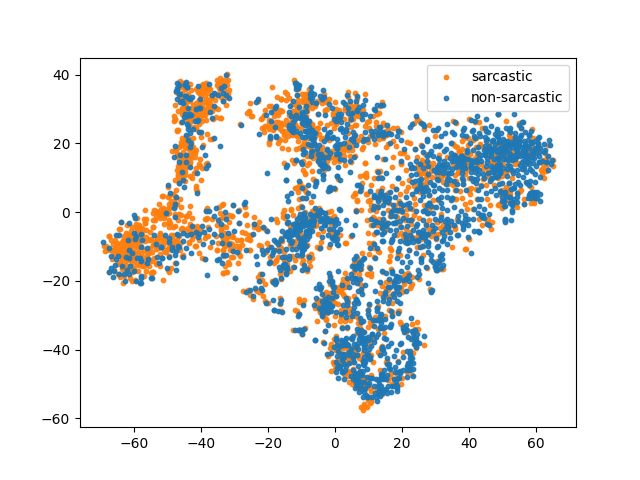
\includegraphics[width=\linewidth]{./figure/tsne_sarc_pol.png}
		 \subcaption{皮肉・非皮肉}
	\end{center}
%		\label{fig:40_tsne1-1}
	\end{minipage}
 	\begin{minipage}{0.4\hsize}
	\begin{center}
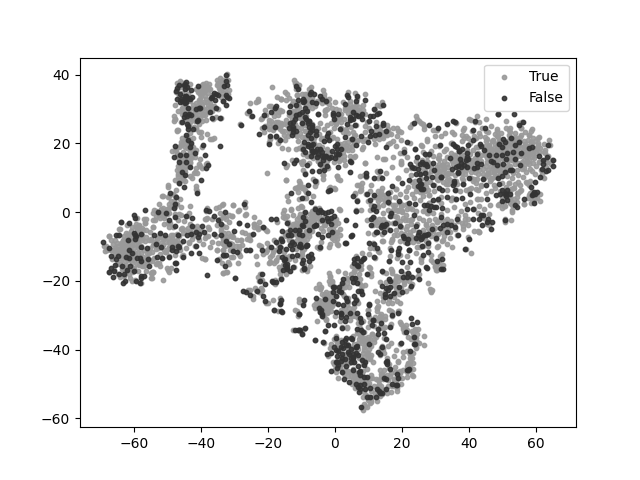
\includegraphics[width=\linewidth]{./figure/tsne_TorF_pol.png}
		\subcaption{正解・不正解}
 	 \end{center}
%		\label{fig:40_tsne1-2}
 	\end{minipage}
	\caption{t-SNE による可視化 (politics)}
	\label{fig:40_tsne1}
\end{center}
\end{figure}
% end figure

%%% figure minipage
\begin{figure}[tb]
\begin{center}
 	\begin{minipage}{0.4\hsize}
	\begin{center}
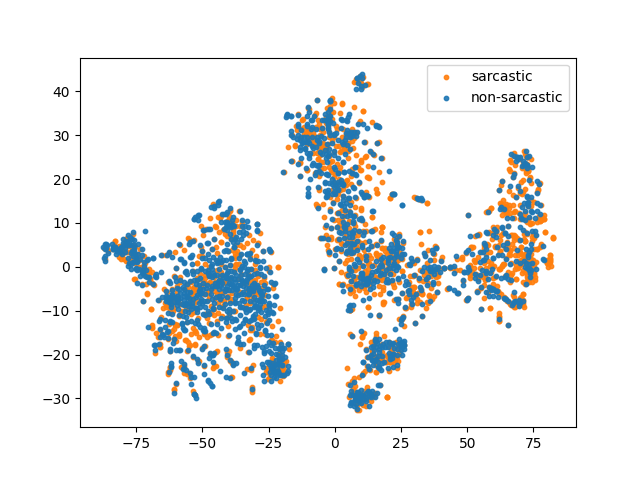
\includegraphics[width=\linewidth]{./figure/tsne_sarc_ask.png}
		 \subcaption{皮肉・非皮肉}
	\end{center}
%		\label{fig:40_tsne2-1}
	\end{minipage}
 	\begin{minipage}{0.4\hsize}
	\begin{center}
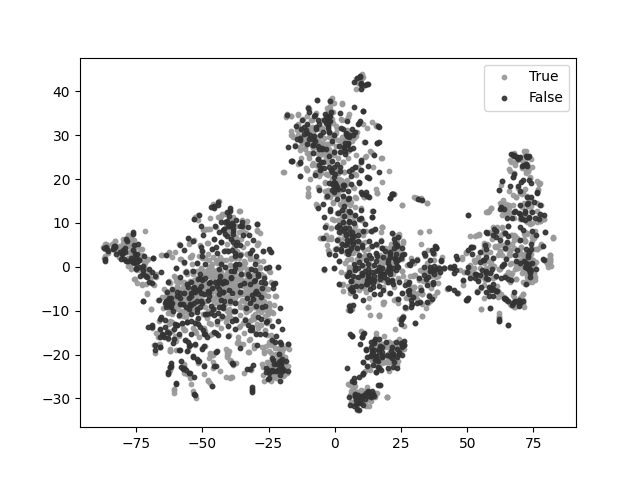
\includegraphics[width=\linewidth]{./figure/tsne_TorF_ask.png}
		\subcaption{正解・不正解}
 	 \end{center}
%		\label{fig:40_tsne2-2}
 	\end{minipage}
	\caption{t-SNE による可視化 (AskReddit)}
	\label{fig:40_tsne2}
\end{center}
\end{figure}
% end figure

%%% figure minipage
\begin{figure}[tb]
\begin{center}
 	\begin{minipage}{0.4\hsize}
	\begin{center}
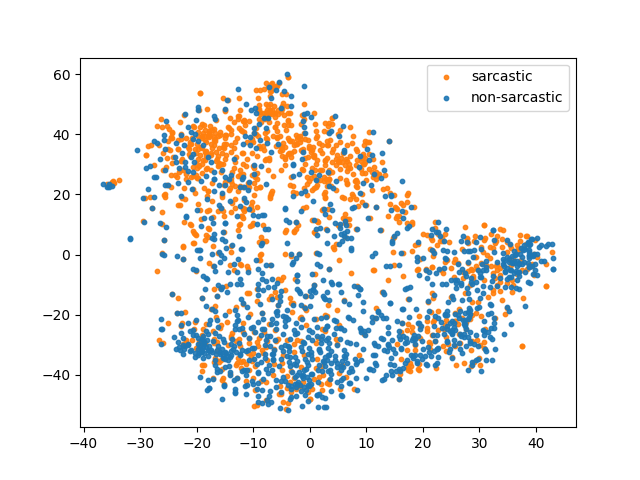
\includegraphics[width=\linewidth]{./figure/tsne_sarc_world.png}
		 \subcaption{皮肉・非皮肉}
	\end{center}
%		\label{fig:40_tsne3-1}
	\end{minipage}
 	\begin{minipage}{0.4\hsize}
	\begin{center}
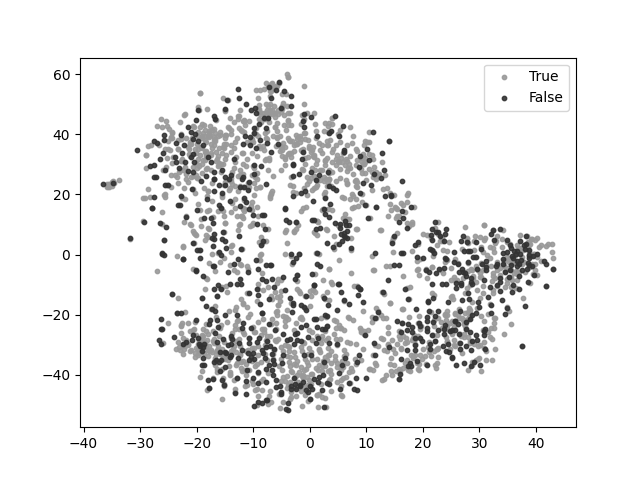
\includegraphics[width=\linewidth]{./figure/tsne_TorF_world.png}
		\subcaption{正解・不正解}
 	 \end{center}
%		\label{fig:40_tsne3-2}
 	\end{minipage}
	\caption{t-SNE による可視化 (worldnews)}
	\label{fig:40_tsne3}
\end{center}
\end{figure}
% end figure

%%% figure minipage
\begin{figure}[tb]
\begin{center}
 	\begin{minipage}{0.4\hsize}
	\begin{center}
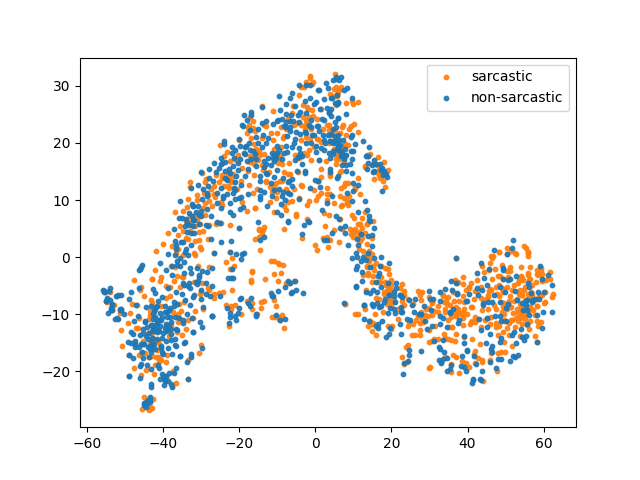
\includegraphics[width=\linewidth]{./figure/tsne_sarc_pc.png}
		 \subcaption{皮肉・非皮肉}
	\end{center}
%		\label{fig:40_tsne4-1}
	\end{minipage}
 	\begin{minipage}{0.4\hsize}
	\begin{center}
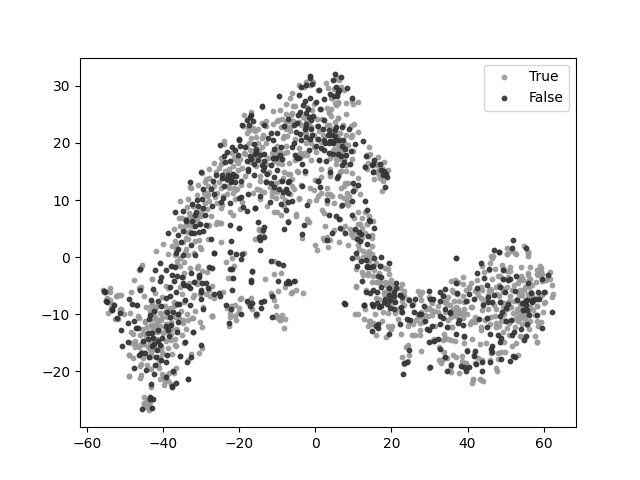
\includegraphics[width=\linewidth]{./figure/tsne_TorF_pc.png}
		\subcaption{正解・不正解}
 	 \end{center}
%		\label{fig:40_tsne4-2}
 	\end{minipage}
	\caption{t-SNE による可視化 (pcmasterrace)}
	\label{fig:40_tsne4}
\end{center}
\end{figure}
% end figure

%%% figure minipage
\begin{figure}[tb]
\begin{center}
 	\begin{minipage}{0.4\hsize}
	\begin{center}
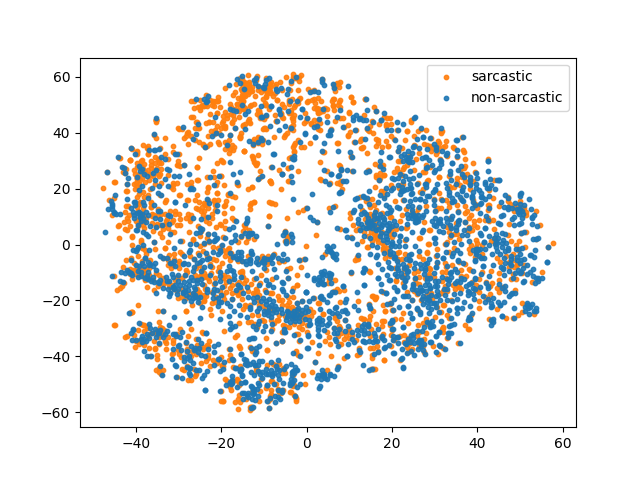
\includegraphics[width=\linewidth]{./figure/tsne_sarc_random.png}
		 \subcaption{皮肉・非皮肉}
	\end{center}
%		\label{fig:40_tsne4-1}
	\end{minipage}
 	\begin{minipage}{0.4\hsize}
	\begin{center}
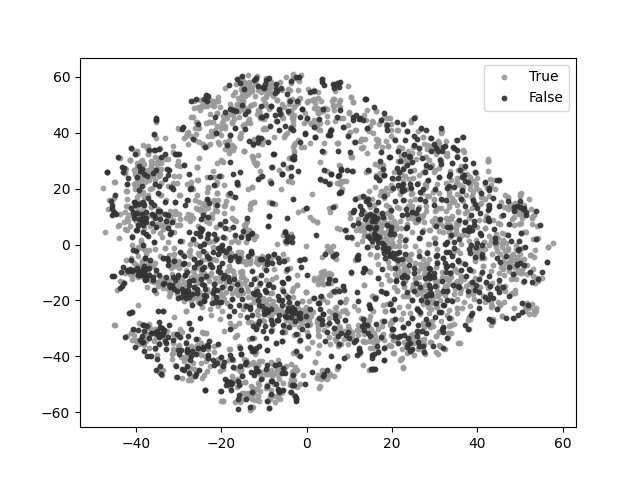
\includegraphics[width=\linewidth]{./figure/tsne_TorF_random.png}
		\subcaption{正解・不正解}
 	 \end{center}
%		\label{fig:40_tsne4-2}
 	\end{minipage}
	\caption{t-SNE による可視化 (random)}
	\label{fig:40_tsne5}
\end{center}
\end{figure}
% end figure




%%%%%%%%%%%%%%%%%%%%%%%%%%%%%%

%\subsubsection{GlobalOffensive,AskReddit で精度が低下したことへの考察}
%
%まず,各データセットの中身を見てみる.
%
%\begin{enumerate}
%\item[例 1] aaa
%\item[例 2] bbb
%\end{enumerate}





\clearpage

% 5. conclusion
\newpage
\changeindent{0cm}
\section{まとめと今後の課題}
\changeindent{2cm}

%まとめ
本研究では皮肉推定の前段階として,文章の話題ごとの皮肉推定の有効性を検証した.
Reddit における投稿トピック subreddit のそれぞれについて皮肉推定した結果,皮肉表現を一括りに扱って推定するよりも推定精度が向上することが確認できた.

%今後の課題
今後の課題として,本研究での成果を踏まえ,各話題ごとに学習した皮肉推定モデルを組み合わせたアンサンブル学習によって,データセット全体に対する皮肉推定に取り組むことが挙げられる.
また皮肉推定に使用する文脈情報やメタデータを拡大することにより,推定精度の向上を目指す.

% shaji
\clearpage
\newpage
\changeindent{0cm}
\acknowledgements
\changeindent{2cm}
本研究を進めるにあたり,御指導,御鞭撻を賜りました森直樹教授に深く感謝の意を表します.岡田真助教には直接御指導頂き,研究方針を初めとした多大な御助言を頂きました.心より御礼申し上げます.\par
諸先輩方からは研究に関して建設的な意見を頂きました.また同期の皆さんとは共に切磋琢磨し励ましあいながら研究に取り組みました.心より感謝致します.\par


\begin{flushright}
 2022 年 2 月 25 日
\end{flushright}
  % shaji

% References
\clearpage
\newpage
\changeindent{0cm}
\begin{thebibliography}{99}
\changeindent{2cm}



% irony 1
\bibitem {GIBBS1991523}
Raymond W. Gibbs and Jennifer O’Brien. 
Psychological aspects of irony understanding. 
Journal of Pragmatics, Vol. 16, No. 6, pp. 523--530, 1991.


% irony 2
\bibitem {HAVERKATE199077}
Henk Haverkate. 
A speech act analysis of irony. 
Journal of Pragmatics, Vol. 14, No. 1, pp. 77--109, 1990.


% irony 3
\bibitem {Ozerova} 
オーゼロヴァ・アナスタシーア.
言語的皮肉の現象についての理論とその原理 : 日本語における皮肉の分析を中心に.
日本語・日本文化研究, Vol. 26, pp. 147--157, 2016.

% twitter 1
% 
\bibitem{DBLP:conf/emnlp/RiloffQSSGH13}
Ellen Riloff, Ashequl Qadir, Prafulla Surve, Lalindra De Silva, Nathan Gilbert, and Ruihong Huang. 
Sarcasm as contrast between a positive sentiment and negative situation. 
In EMNLP, pp. 704--714, 2013.


% twitter 2
\bibitem{ghosh-veale-2017-magnets}
Aniruddha Ghosh and Tony Veale. 
Magnets for sarcasm: Making sarcasm detection timely, contextual and very personal. 
In Proceedings of the 2017 Conference on Empirical Methods in Natural Language Processing, pp. 482--491, Copenhagen, Denmark, September 2017. Association for Computational Linguistics.


% news headlines dataset 
\bibitem {misra2019sarcasm}
Rishabh Misra and Prahal Arora. 
Sarcasm detection using hybrid neural network. 
2019.


% SARC データセット
% https://aclanthology.org/L18-1102/
\bibitem {khodak2018}
Mikhail Khodak, Nikunj Saunshi, and Kiran Vodrahalli.
A Large Self-Annotated Corpus for Sarcasm.
In Proceedings of the Eleventh International Conference on Language Resources and Evaluation (LREC 2018), Miyazaki, Japan, May, 2018. European Language Resources Association (ELRA).


% CASCADE 
% https://aclanthology.org/C18-1156/
\bibitem {hazarika-etal-2018-cascade}
Devamanyu Hazarika, Soujanya Poria, Sruthi Gorantla, Erik Cambria, Roger Zimmermann, and Rada Mihalcea.
CASCADE: Contextual Sarcasm Detection in Online Discussion Forums.
In Proceedings of the 27th International Conference on Computational Linguistics, pp. 1837--1848, Santa Fe, New Mexico, USA, August 2018. Association for Computational Linguistics.


% Deep and Dense Sarcasm Detection
% https://arxiv.org/abs/1911.07474
\bibitem {pelser2019deep}
Devin Pelser and Hugh Murrell.
Deep and dense sarcasm detection.
2019.



% BERT 
% https://aclanthology.org/L18-1102
\bibitem {devlin-etal-2019-bert}
Jacob Devlin, Ming-Wei Chang, Kenton Lee, and Kristina Toutanova.
BERT: Pre-training of Deep Bidirectional Transformers for Language Understanding.
In Proceedings of the 2019 Conference of the North American Chapter of the Association for Computational Linguistics: Human Language Technologies, Volume 1 (Long and Short Papers), pp. 4171--4186, Minneapolis, Minnesota, June 2019. Association for Computational Linguistics.


% Transformer
% https://papers.nips.cc/paper/2017/file/3f5ee243547dee91fbd053c1c4a845aa-Paper.pdf
\bibitem {NIPS2017_3f5ee243}
Ashish Vaswani, Noam Shazeer, Niki Parmar, Jakob Uszkoreit, Llion Jones, Aidan N Gomez, \L ukasz Kaiser, and Illia Polosukhin.
Attention is all you need.
2017.
In Advances in Neural Information Processing Systems, Vol. 30.


% BookCorpus
% https://www.computer.org/csdl/proceedings-article/iccv/2015/8391a019/12OmNro0HYa
\bibitem {bookcorpus}
Yukun Zhu, Ryan Kiros, Rich Zemel, Ruslan Salakhut- dinov, Raquel Urtasun, Antonio Torralba, and Sanja Fidler.
Aligning books and movies: Towards story-like visual explanations by watching movies and reading books. 
In Proceedings of the IEEE international conference on computer vision (ICCV 2015), pp 19--27, Los Alamitos, CA, USA, December 2015. IEEE Computer Society.


% WordPiece
% https://arxiv.org/abs/1609.08144
\bibitem {wu2016googles}
Yonghui Wu, Mike Schuster, Zhifeng Chen, Quoc V. Le, Mohammad Norouzi, Wolfgang Macherey, Maxim Krikun, Yuan Cao, Qin Gao, Klaus Macherey, Jeff Klingner, Apurva Shah, Melvin Johnson, Xiaobing Liu, \L ukasz Kaiser, Stephan Gouws, Yoshikiyo Kato, Taku Kudo, Hideto Kazawa, Keith Stevens, George Kurian, Nishant Patil, Wei Wang, Cliff Young, Jason Smith, Jason Riesa, Alex Rudnick, Oriol Vinyals, Greg Corrado, Macduff Hughes, and Jeffrey Dean.
Google's Neural Machine Translation System: Bridging the Gap between Human and Machine Translation.
2016.


% Optuna
% https://github.com/optuna/optuna
\bibitem {akiba2019optuna}
Takuya Akiba, Shotaro Sano, Toshihiko Yanase, Takeru Ohta, and Masanori Koyama.
Optuna: A Next-generation Hyperparameter Optimization Framework.
In Proceedings of the 25th ACM SIGKDD International Conference on Knowledge Discovery \& Data Mining, KDD ’19, pp. 2623--2631, New York, NY, USA, 2019. Association for Computing Machinery.


% t-SNE
% 
\bibitem {JMLR:v9:vandermaaten08a}
Laurens van der Maaten and Geoffrey Hinton. 
Visualizing Data using t-SNE. 
Journal of Machine Learning Research, Vol. 9, No. 86, pp. 2579--2605, 2008.





\end{thebibliography}

% 参考文献(thebibliography)については iepaper.sty の line 112 ~ 116 で定義されている.
% README 読む分には,bibitem で書くみたい.
% 1つ1つ手打ちする必要があるので,卒論の参考文献のフォーマット等があるかどうか調べておく




\end{document}
